\chapter{پاکسازی داده‌ها و مهندسی ویژگی‌ها}

\section{پاکسازی داده‌ها} داده‌های خام مورد استفاده در این پژوهش از دو منبع اصلی استخراج شده‌اند: \begin{itemize}
    \item \textbf{فایل‌های سالم} (\lr{benign.csv}) با ۳۵۴ نمونه
    \item \textbf{فایل‌های آلوده} (\lr{ransom.csv}) با ۱۱۹ نمونه
\end{itemize}

در بررسی اولیه، چند چالش اصلی شناسایی گردید:
\begin{itemize}
    \item \textbf{عدم یکپارچگی فرمت‌ها:} نام فایل‌ها در ستون \lr{NAME} به‌صورت ویندوزی و یونیکسی ذخیره شده بود.
    \item \textbf{مقادیر گمشده:} حدود ۱۲ درصد از مقادیر ستون‌های \lr{rwxc} و \lr{rwx} ثبت نشده بودند.
    \item \textbf{وجود ستون‌های اضافی:} برخی ستون‌ها مانند \lr{MD5\_HASH} و \lr{SHA256\_HASH} برای تحلیل رفتار فایل ضروری نبودند.
\end{itemize}

برای رفع این چالش‌ها، فرایند پاکسازی در سه مرحله به‌طور جامع انجام شد:

\subsection{۱. پاکسازی ساختاری}
\begin{itemize}
    \item حذف ستون‌های غیرمرتبط (مانند \lr{ID, DATEADDED, CUCKOO\_ID}).
    \item یکسان‌سازی مسیر فایل‌ها؛ به‌عنوان مثال، با جداسازی قسمت نهایی مسیر:
    \begin{verbatim}
        df['LOCATION'] = df['LOCATION'].str.split('\\').str[-1]
    \end{verbatim}
\end{itemize}

\subsection{۲. مدیریت مقادیر گمشده}
\begin{itemize}
    \item جایگزینی مقادیر عددی با میانه‌ی ستون مربوطه.
    \item حذف سطرهایی که بیش از ۳۰\% از داده‌های آن‌ها نامشخص بوده است.
\end{itemize}

\subsection{۳. تبدیل داده‌های نمادین}
\begin{itemize}
    \item تبدیل اعداد فارسی به انگلیسی در ستون‌های عددی.
    \item استانداردسازی برچسب‌ها؛ به‌عنوان مثال، دسته‌بندی یکدست مقادیر ستون \lr{CATEGORY} به ۵ کلاس اصلی.
\end{itemize}

پس از اعمال این مراحل، داده‌ها از نظر ساختاری تمیز و یکپارچه شده و برای مراحل بعدی آماده شدند.

\section{مهندسی ویژگی‌ها} هدف از مهندسی ویژگی‌ها، استخراج اطلاعات عمیق و الگوهای پنهان در رفتار دسترسی به فایل‌ها است. به همین منظور، چندین ویژگی ترکیبی بر مبنای مجوزهای دسترسی پایه استخراج شدند. در ادامه، به معرفی این ویژگی‌های جدید و فرمول‌های مربوط به آن‌ها می‌پردازیم:

\subsection{ویژگی‌های ترکیبی استخراج‌شده}
\begin{itemize}
    \item \textbf{نسبت نوشتن (\lr{write\_ratio}):}
    \begin{equation}
        \text{\lr{write\_ratio}} = \frac{rw}{r+1}
    \end{equation}
    این شاخص به‌منظور شناسایی فعالیت‌های نوشتن مکرر و غیرعادی در فایل‌ها طراحی شده است.

    \item \textbf{نسبت اجرا (\lr{execute\_ratio}):}
    \begin{equation}
        \text{\lr{execute\_ratio}} = \frac{rx}{r+1}
    \end{equation}
    این ویژگی با تمرکز بر فرکانس اجرای فایل، احتمال رفتار مخرب در فایل‌های اجرایی را مورد بررسی قرار می‌دهد.

    \item \textbf{امتیاز پیچیدگی (\lr{complexity\_score}):}
    \begin{equation}
        \text{\lr{complexity\_score}} = \log_{10}(rwxc+1) \times \sqrt{rwx}
    \end{equation}
    این شاخص با ترکیب لگاریتم و ریشه دوم، توانایی تشخیص الگوهای پیچیده در دسترسی به فایل‌ها را فراهم می‌کند.

    \item \textbf{وزن دسترسی (\lr{weighted\_perm}):}
    \begin{equation}
        \text{\lr{weighted\_perm}} = 0.3r + 0.2rw + 0.15rx + 0.1rwc + 0.15rwx + 0.1rwxc
    \end{equation}
    ضرایب انتخاب‌شده بر مبنای اهمیت هر مجوز در تحلیل اولیه با استفاده از مدل \lr{Random Forest} تعیین گردید.
\end{itemize}

\subsection{تحلیل آماری و انتخاب نهایی ویژگی‌ها} برای ارزیابی عملکرد و ارتباط ویژگی‌های استخراج‌شده، از چند روش تحلیلی بهره گرفته شد:
\begin{itemize}
    \item \textbf{تحلیل همبستگی:} با رسم ماتریس همبستگی (شکل \ref{fig:feature_correlations})، روابط بین ویژگی‌های پایه و ترکیبی مورد بررسی قرار گرفت. این تحلیل به شناسایی ویژگی‌های همخط (مانند \lr{rwx} و \lr{complexity\_score} با همبستگی حدود ۰.۸) کمک کرد.

    \item \textbf{اهمیت ویژگی‌ها:} با استفاده از الگوریتم‌های \lr{Random Forest} و \lr{XGBoost}، اهمیت نسبی هر ویژگی از دو منظر \lr{feature importance} و \lr{permutation importance} سنجیده شد.
\end{itemize}

\begin{figure}[ht]
    \centering
    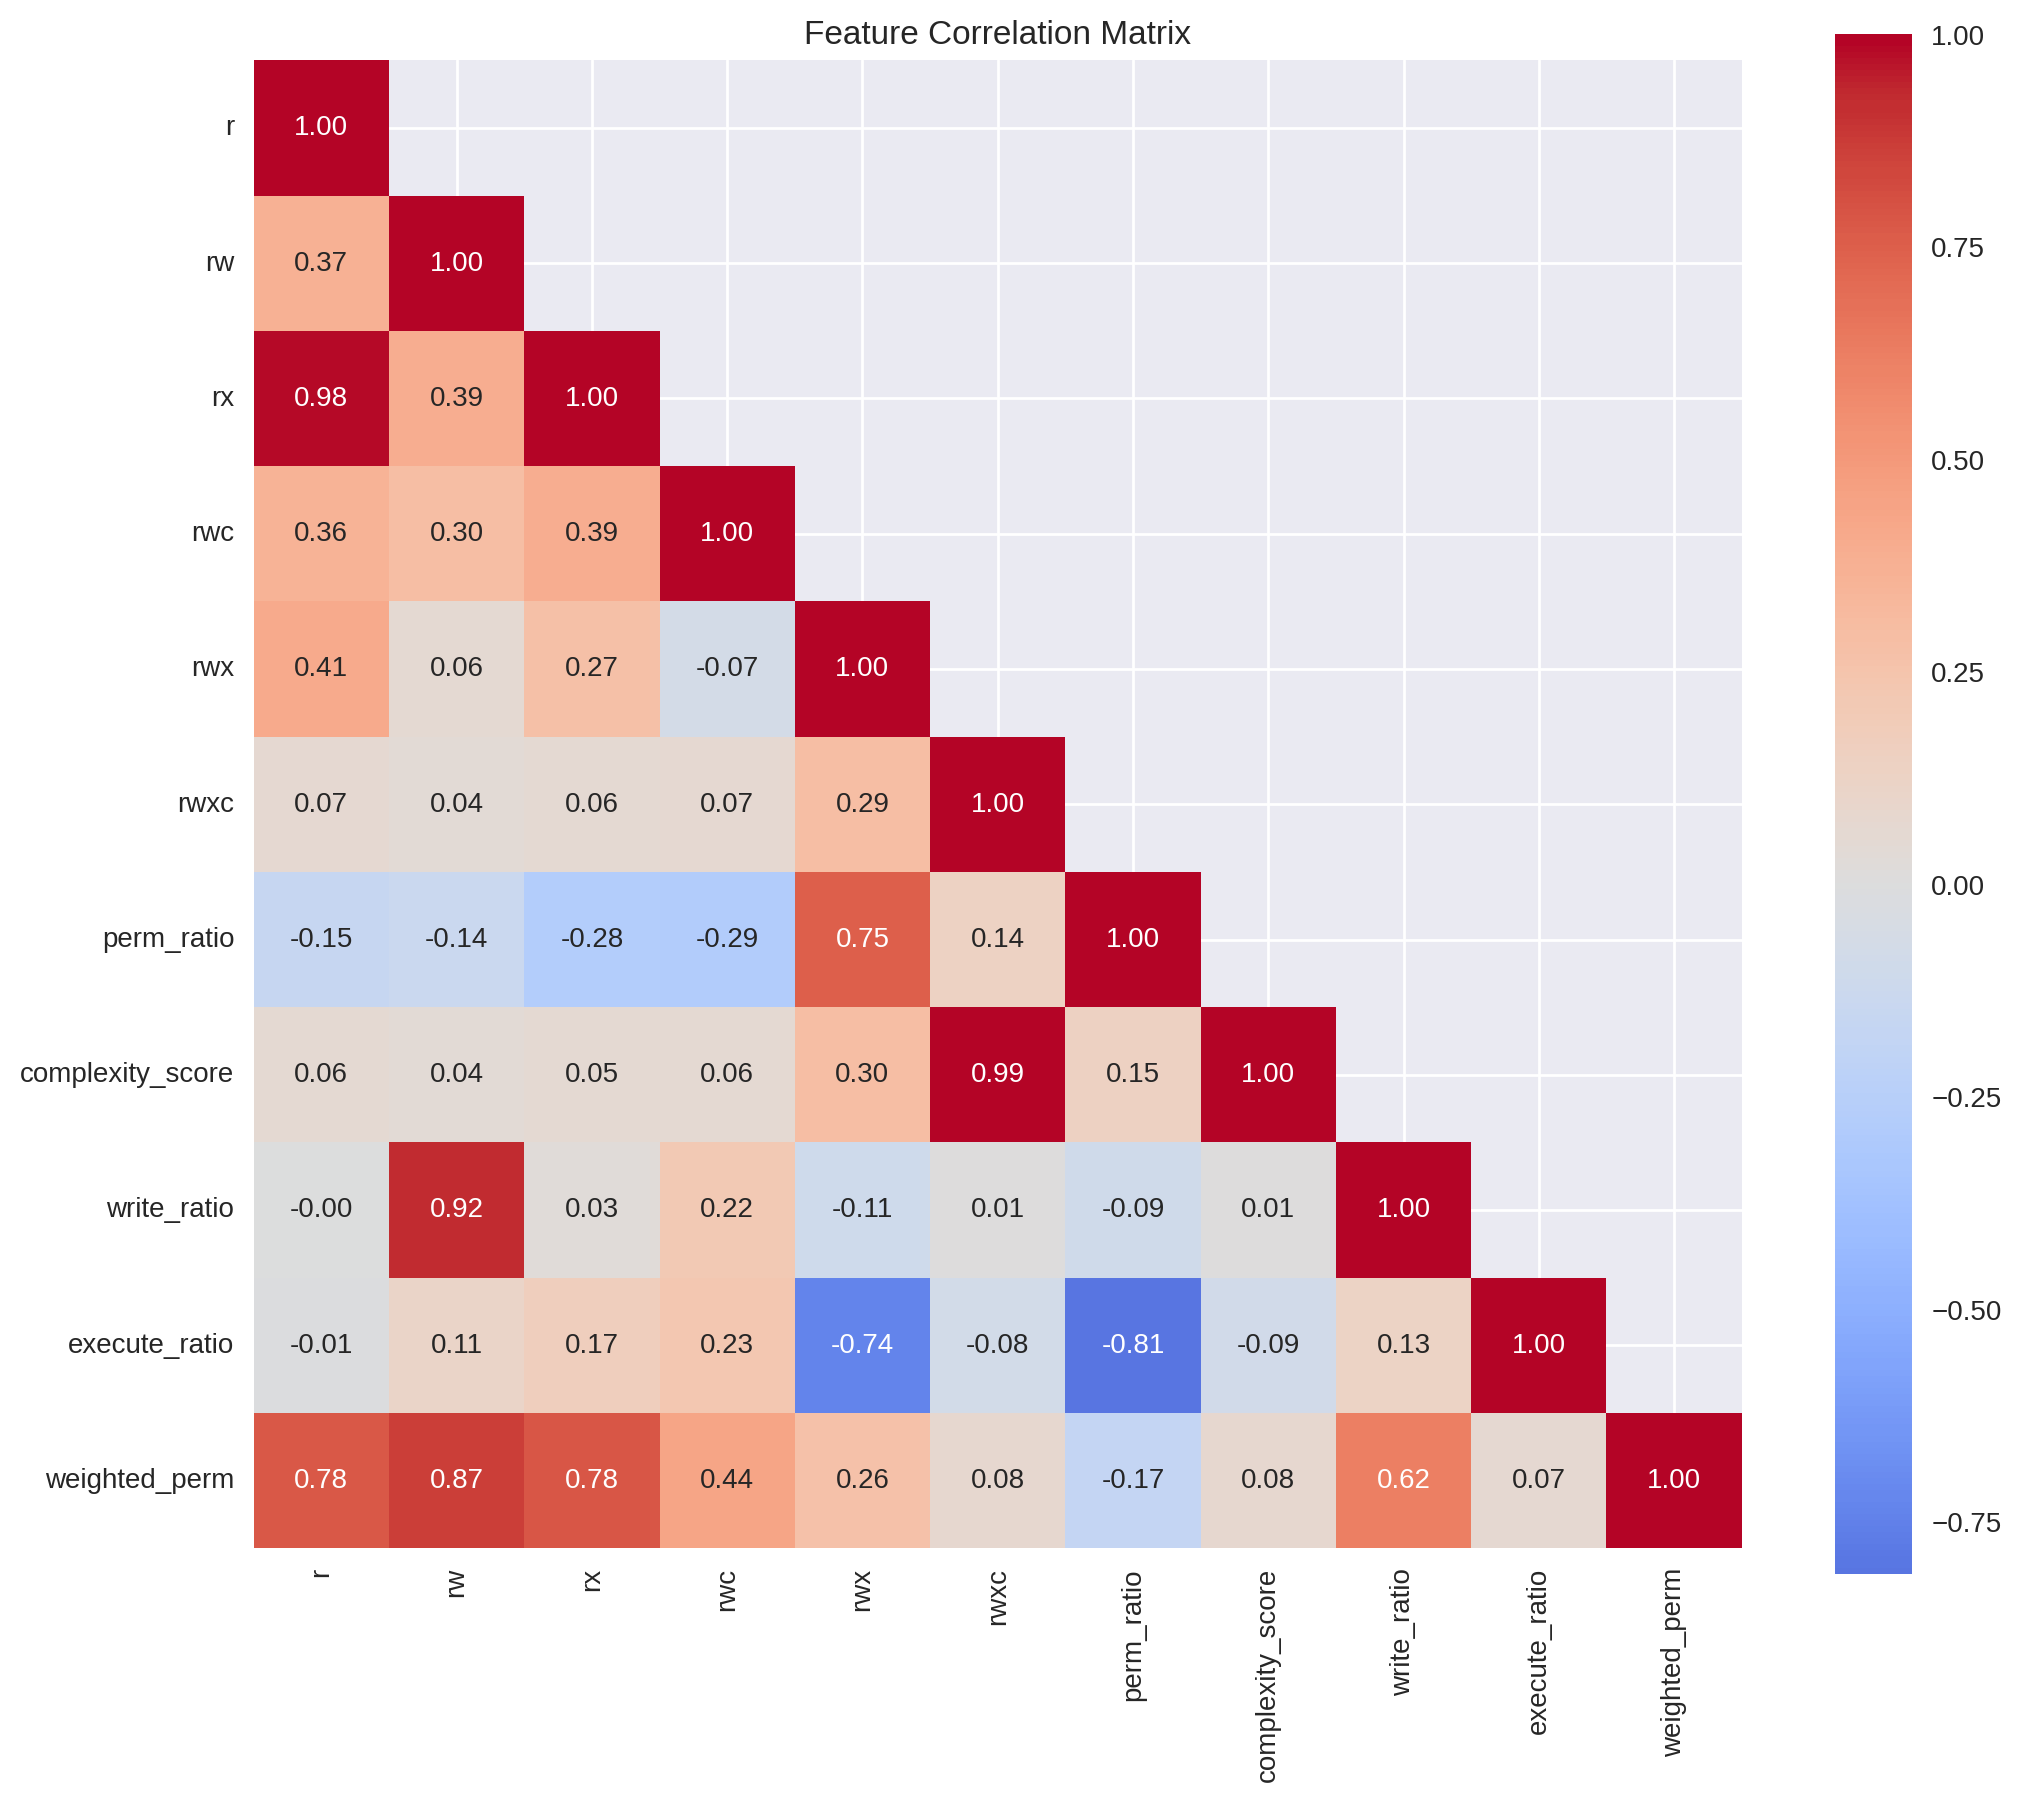
\includegraphics[width=0.8\textwidth]{images/feature_correlations.png}
    \caption{ماتریس همبستگی میان ویژگی‌های استخراج‌شده}
    \label{fig:feature_correlations}
\end{figure}

\subsection{ارائه نتایج تحلیل ویژگی‌ها} تصاویر زیر نتایج استخراج و ارزیابی ویژگی‌های جدید را نشان می‌دهند:
\begin{itemize}
    \item \textbf{اهمیت ویژگی‌ها در مدل \lr{Random Forest}:}
    \begin{figure}[ht]
        \centering
        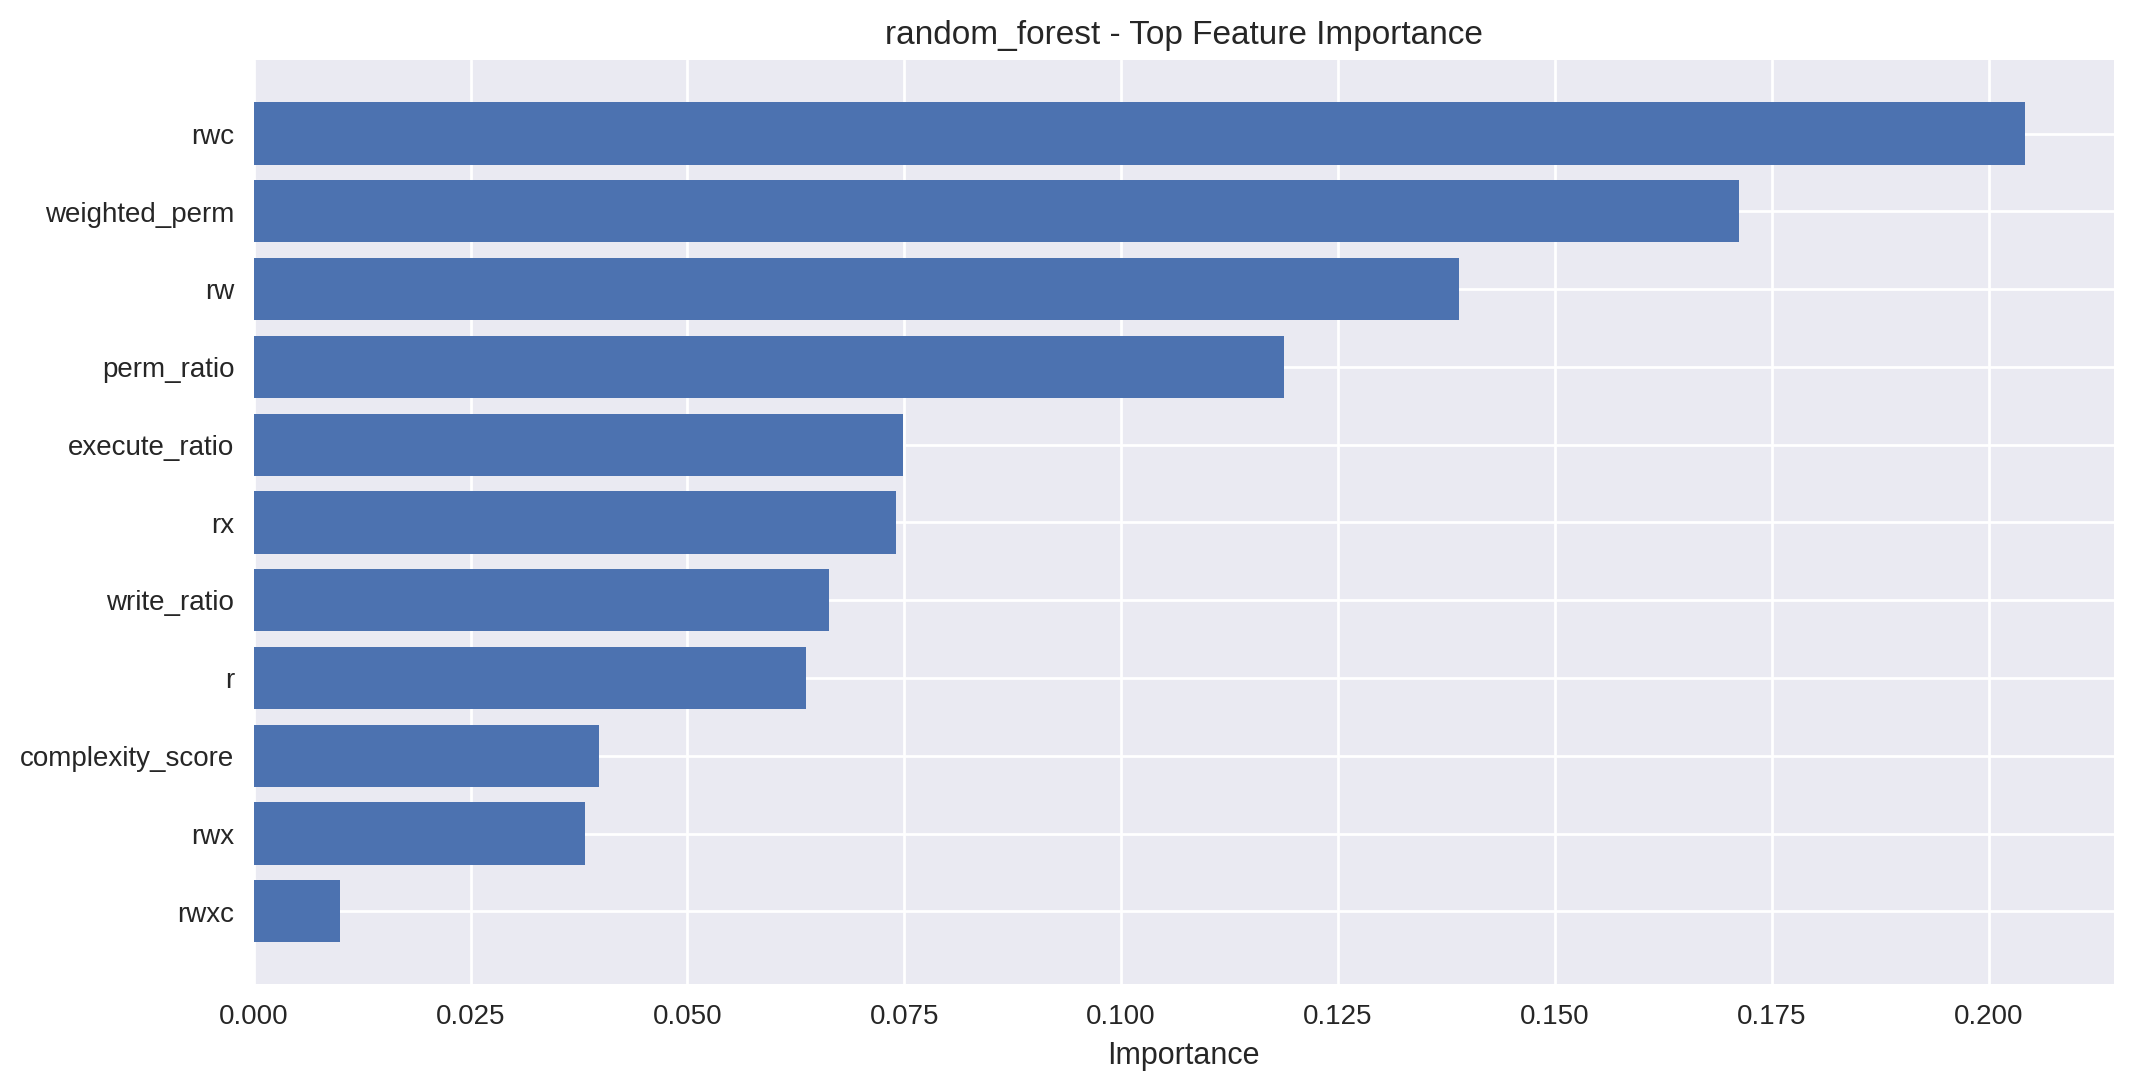
\includegraphics[width=0.7\textwidth]{images/random_forest_feature_importance.png}
        \caption{گراف اهمیت ویژگی‌ها بر مبنای مدل \lr{Random Forest}}
    \end{figure}

    \item \textbf{اهمیت ویژگی‌ها از منظر \lr{Permutation Importance} در \lr{Random Forest}:}
    \begin{figure}[ht]
        \centering
        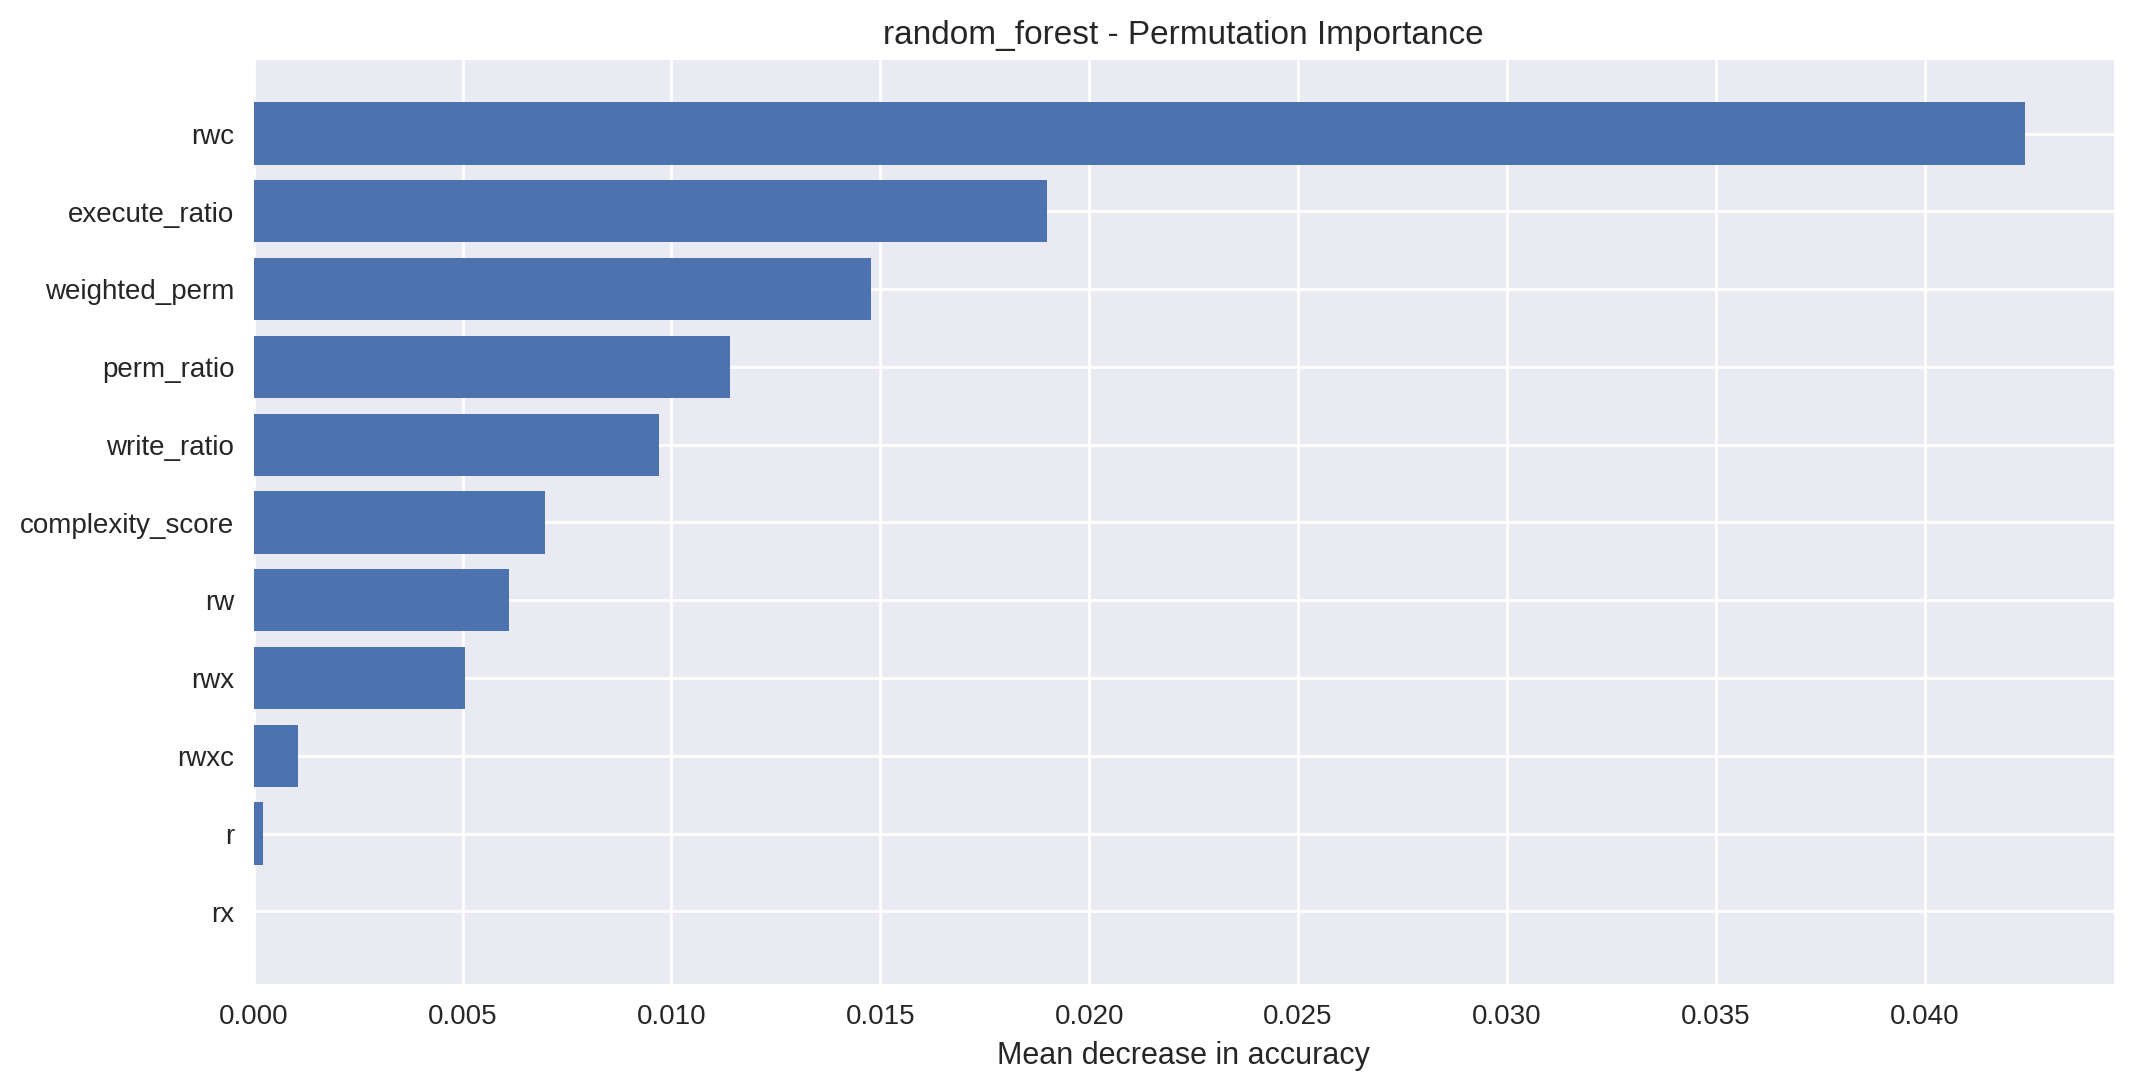
\includegraphics[width=0.7\textwidth]{images/random_forest_permutation_importance.png}
        \caption{تحلیل \lr{Permutation Importance} ویژگی‌ها در مدل \lr{Random Forest}}
    \end{figure}

    \item \textbf{اهمیت ویژگی‌ها در مدل \lr{XGBoost}:}
    \begin{figure}[ht]
        \centering
        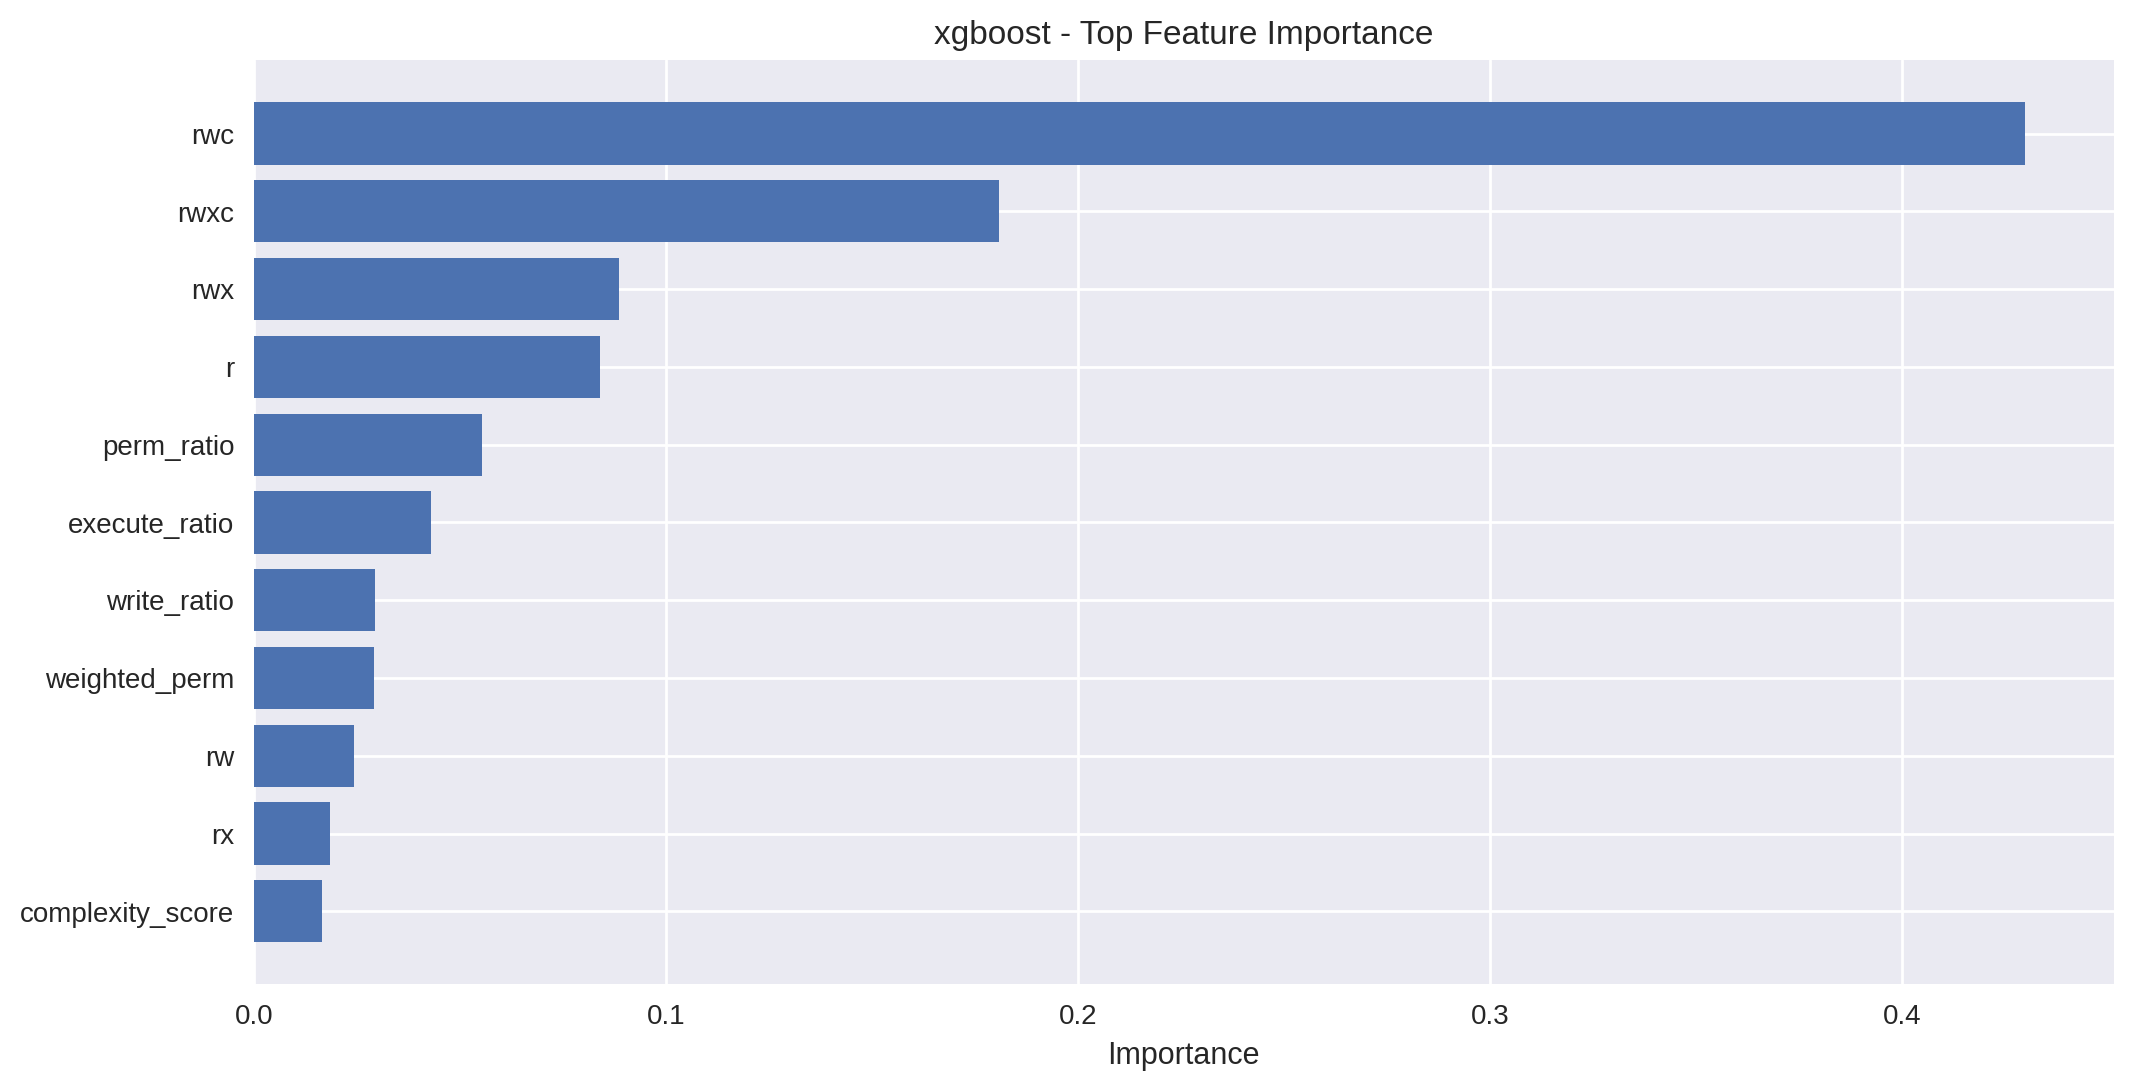
\includegraphics[width=0.7\textwidth]{images/xgboost_feature_importance.png}
        \caption{گراف اهمیت ویژگی‌ها بر مبنای مدل \lr{XGBoost}}
    \end{figure}

    \item \textbf{تحلیل \lr{Permutation Importance} در مدل \lr{XGBoost}:}
    \begin{figure}[ht]
        \centering
        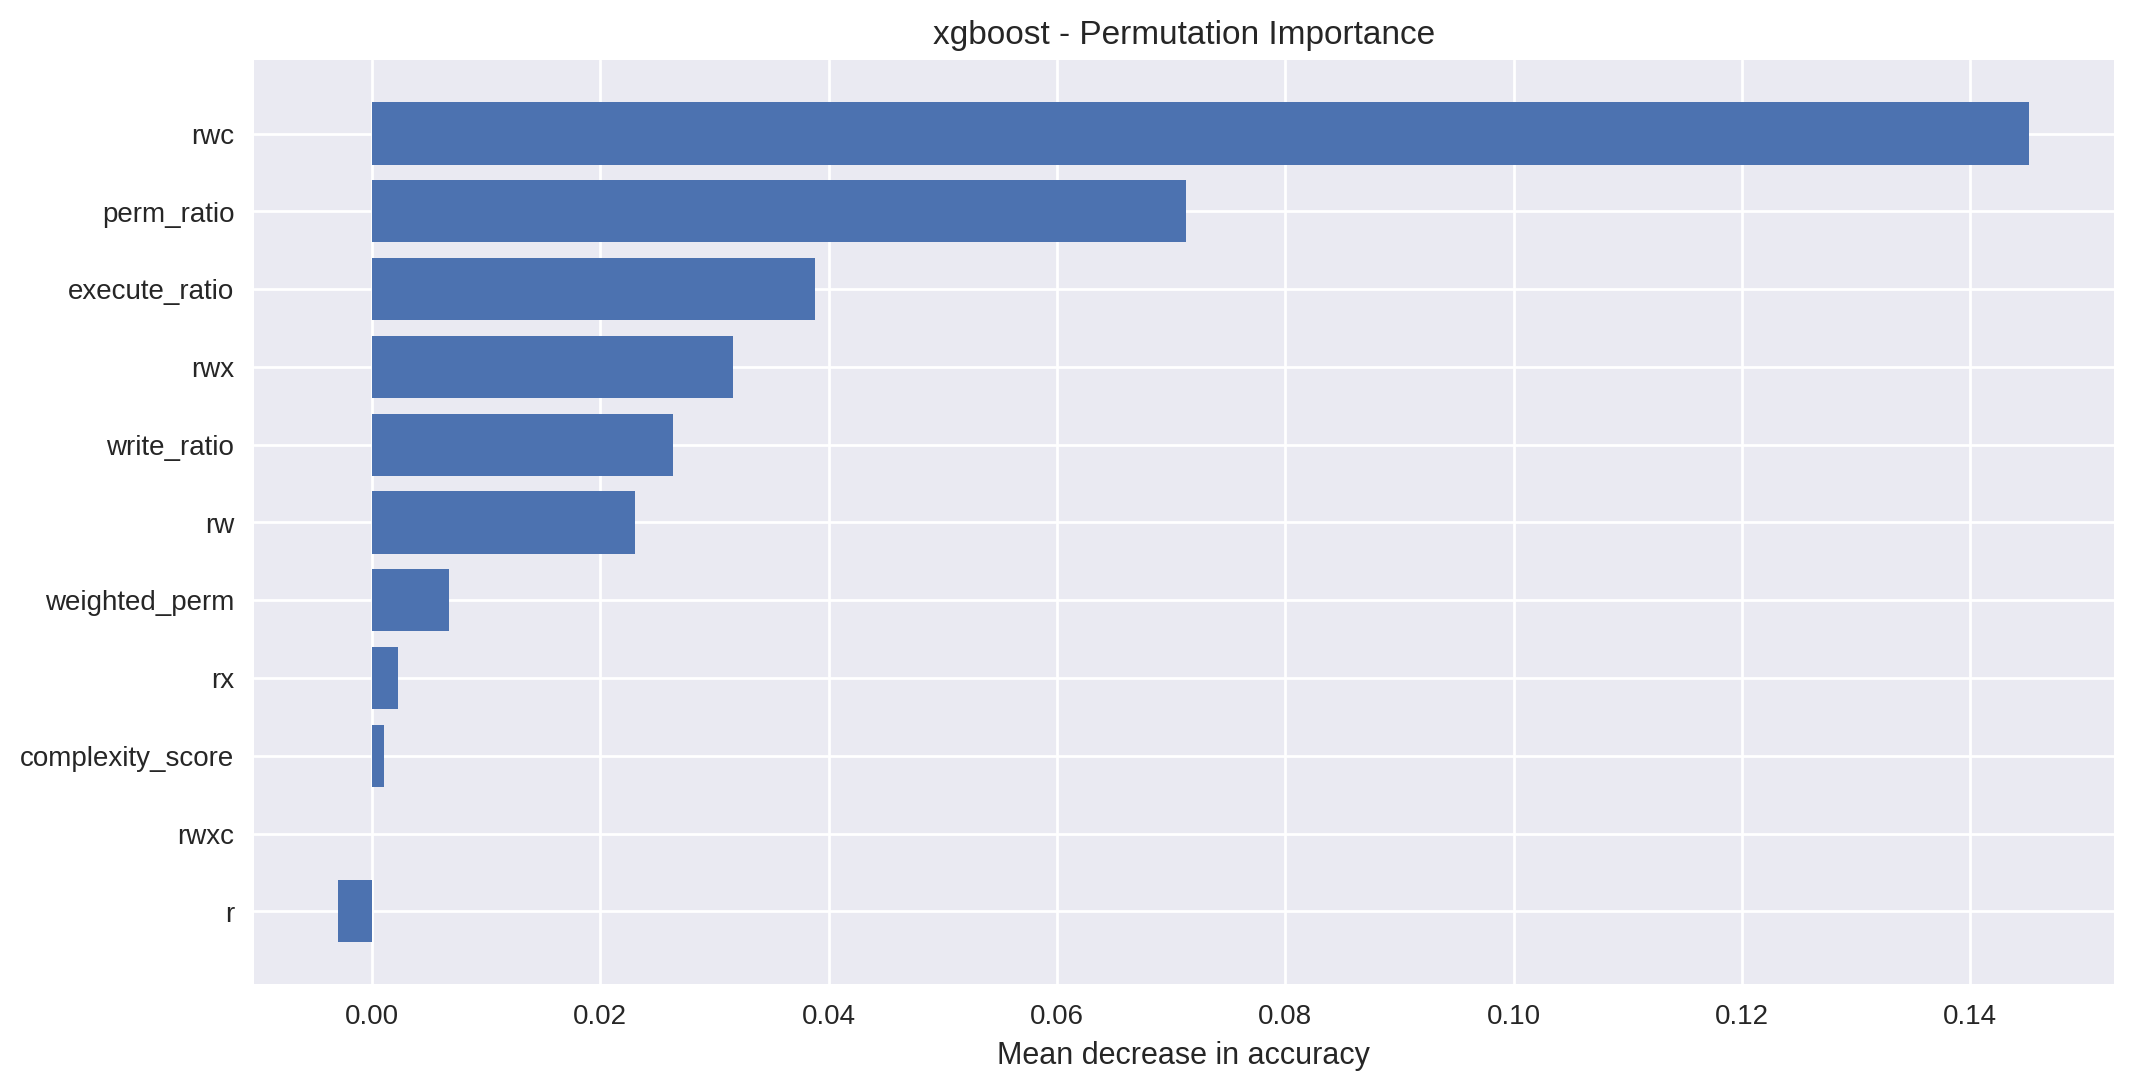
\includegraphics[width=0.7\textwidth]{images/xgboost_permutation_importance.png}
        \caption{ارزیابی \lr{Permutation Importance} ویژگی‌ها در مدل \lr{XGBoost}}
    \end{figure}

    \item \textbf{توزیع ویژگی‌های برتر:}
    \begin{figure}[ht]
        \centering
        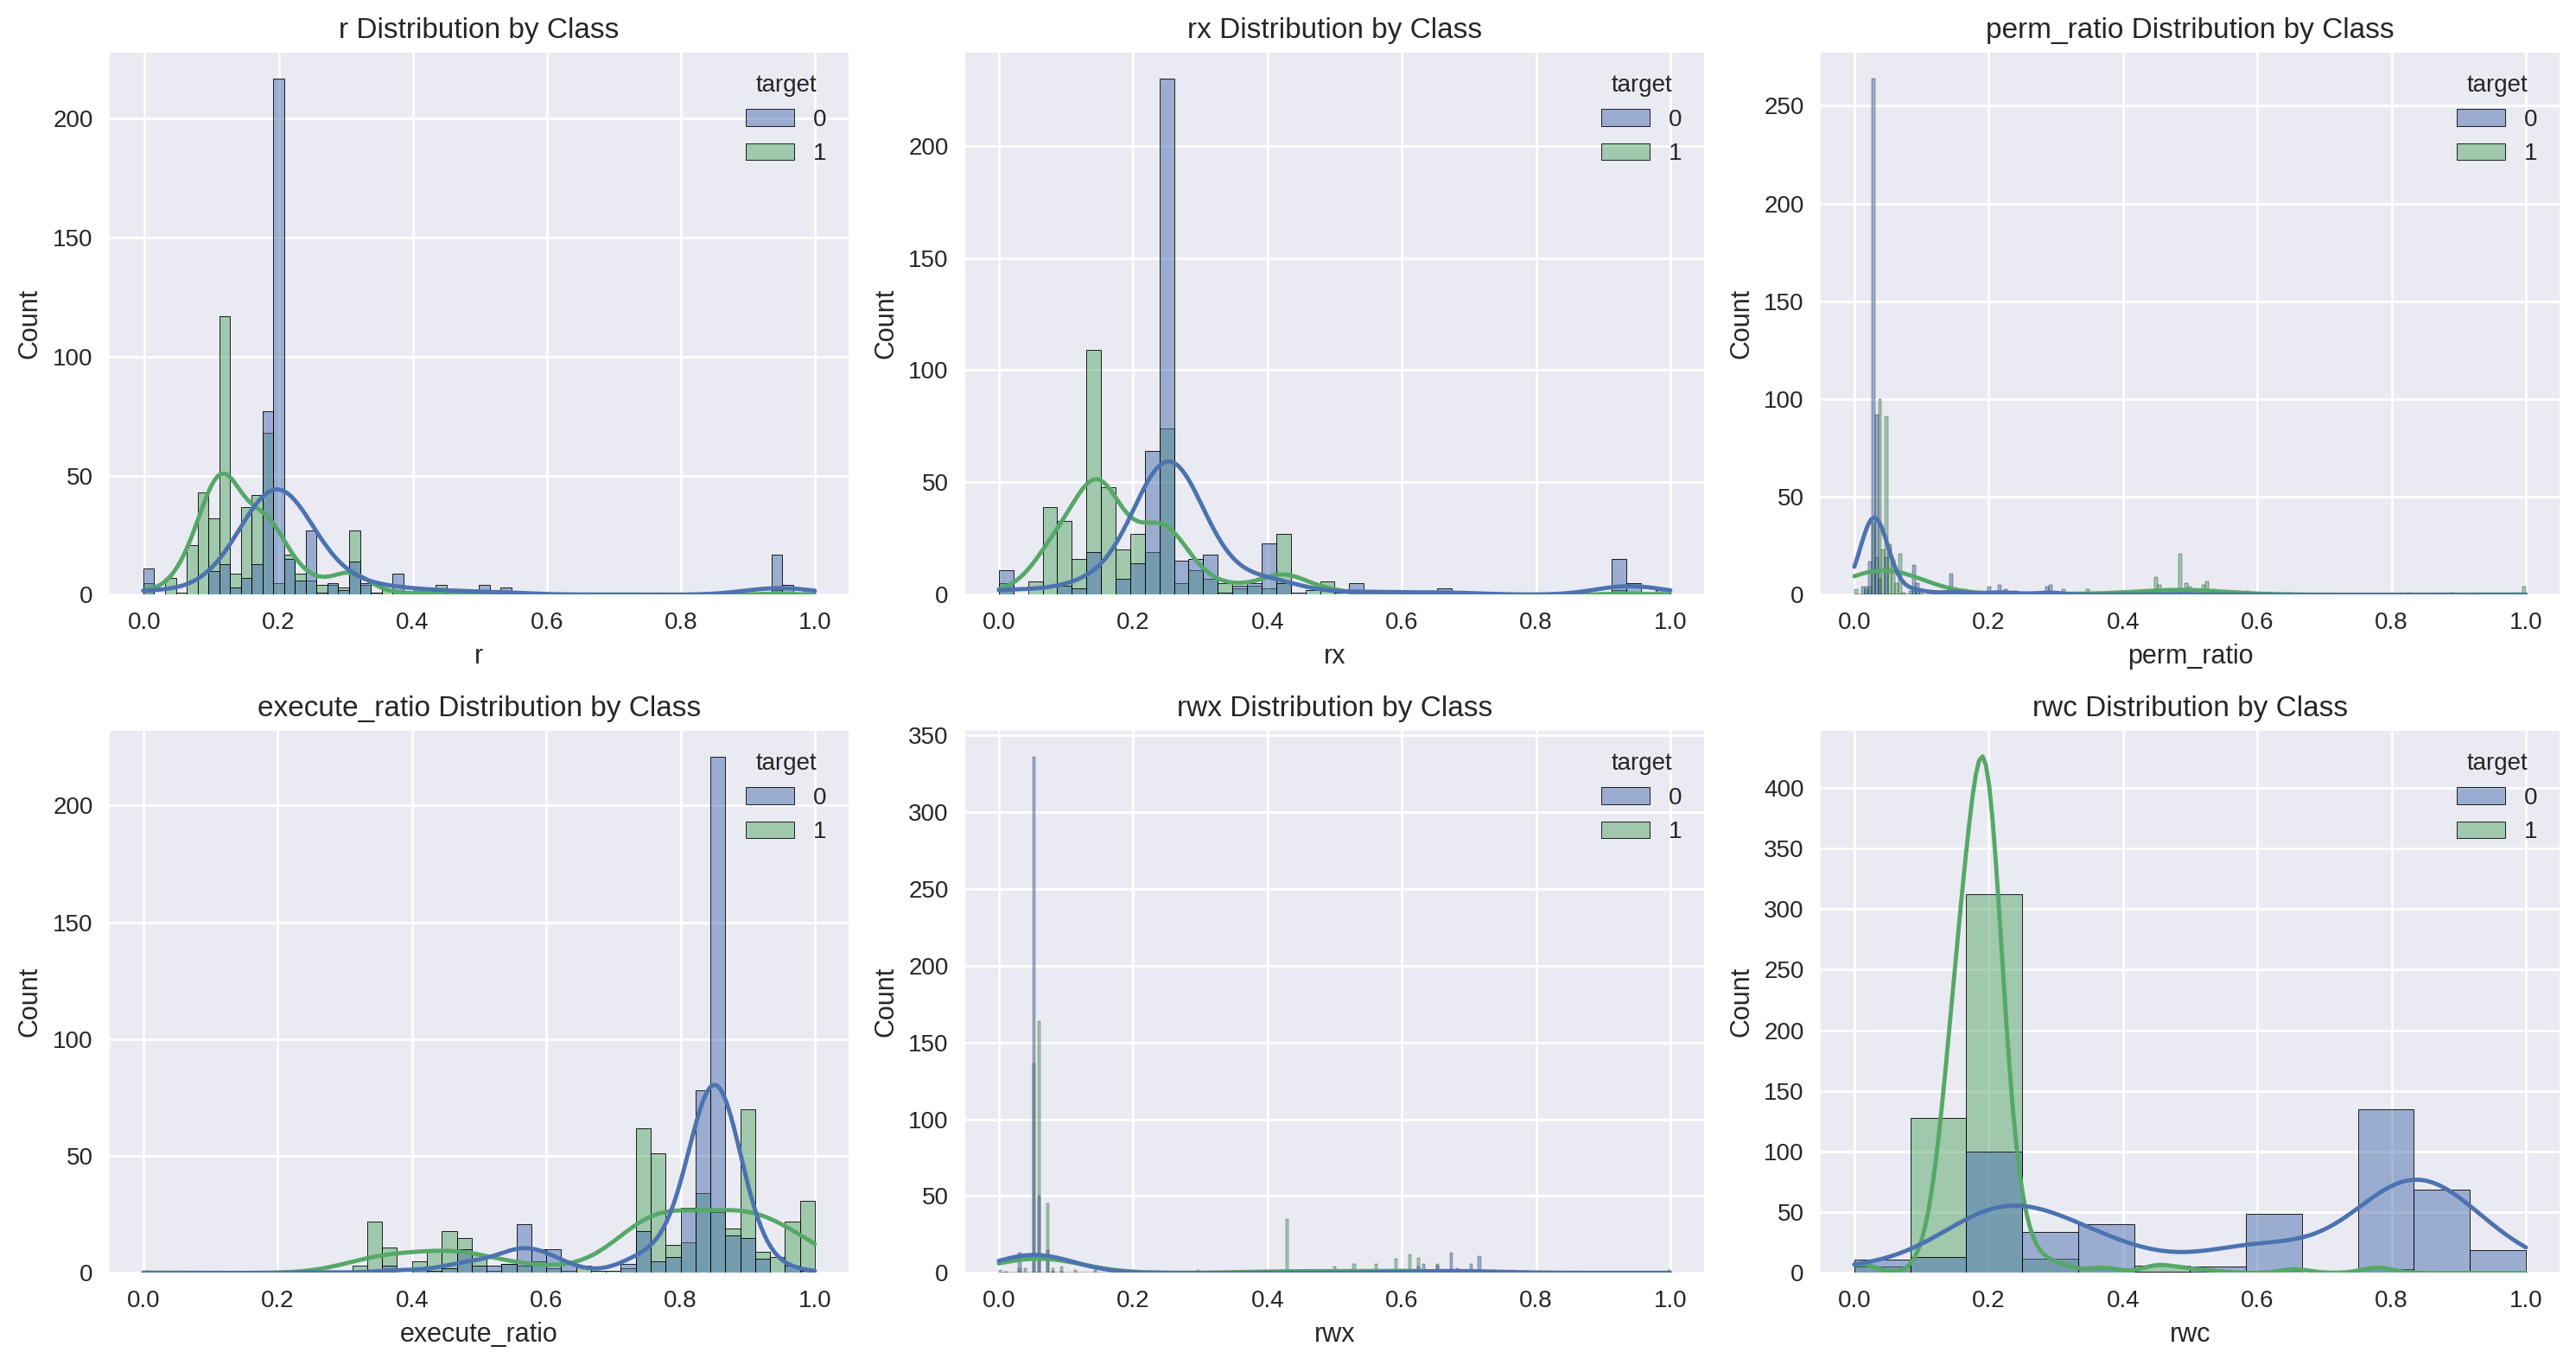
\includegraphics[width=0.7\textwidth]{images/top_feature_distributions.png}
        \caption{توزیع ویژگی‌های منتخب در نمونه‌های مختلف}
    \end{figure}
\end{itemize}

با ارزیابی همبستگی، اهمیت و توزیع ویژگی‌ها، انتخاب نهایی بر روی ویژگی‌هایی مانند \lr{complexity\_score} و \lr{write\_ratio} متمرکز شد تا از بروز مشکلات همخطی جلوگیری گردد. این انتخاب‌ها زمینه‌ی بهینه‌سازی مدل‌های بعدی را فراهم نموده است.

\section{نتیجه‌گیری} پس از انجام دقیق مراحل پاکسازی داده و مهندسی ویژگی، مجموعه‌ی داده به شکلی ساختاریافته و اطلاعات غنی از الگوهای دسترسی به فایل‌ها استخراج گردید. این فرآیند موجب شده تا در فاز مدل‌سازی، داده‌های ورودی از کیفیت بالاتری برخوردار باشند و تاثیر مثبت قابل توجهی در دقت نهایی مدل‌های طبقه‌بندی داشته باشند.

در فصل بعد، به تشریح معماری و روش‌شناسی مدل‌های طبقه‌بندی (از جمله تحلیل عملکرد مدل‌های شبکه عصبی، \lr{Random Forest} و \lr{XGBoost}) پرداخته خواهد شد.